Wie wollen einen Dialog einer graphischen Benutzeroberfläche erstellen, bei der in einem Fenster Daten in Form eines x-y-Graphen angezeigt werden. Die Achensgrößen können durch Klicken im Graphen oder in einem zweiten Fenster durch Eingabe der numerischen Werte verändert werden.
Welches Entwurfsmuster verwenden Sie wie und warum?

\section*{Antwort}
Hierfür eignet sich das \textbf{MVC}-Entwurfsmuster im Zusammenspiel mit dem \code{Observer}-Entwurfsmuster (s. Abbildung~\ref{fig:mvc}).\\

\begin{itemize}
    \item \textbf{Model}: Die \textit{fachlichen Informationen} bestehen aus den \code{x}-\code{y}-Werten der Achse des Graphen und der darzustellenden Daten.\\
    Da auf Zustandsänderungen des Models reagiert werden muss, nimmt das Model die Rolle als \textbf{Observable} (beobachtbar) ein.
    \item \textbf{View}: Die Daten des Models werden in der View repräsentiert: Hierzu existiert in einem Fenster eine Komponente zur Anzeige des Graphen.
    Ein weiteres Fenster zeigt Steuerelemente und Eingabefelder zur Entgegennahme numerischer Werte an.\\
    Die Steuerelemente und Eingabefelder sind \textbf{Observable}, Interaktionen des Nutzers mit ihnen (Mausklick, Tastatureingabe) müssen verarbeitet werden.\\
    Die View-Komponenten beobachten als \textbf{Observer} das Model und aktualisieren die Anzeige, wenn sich der Zustand des Models geändert hat.
    \item \textbf{Controller}: Die Klassen des Controllers reagieren auf Änderungen in der View: Sie verarbeiten die Eingabe numerischer Werte oder reagieren auf Mausereignisse in dem Fenster, das den Graphen enthält.\\
    Daraufhin leitet der Controller die Informationen an das Model weiter, das sich entsprechend aktualisiert.\\
    Die Controller-Klassen sind also auch \textbf{Observer} für \textit{Ereignisse}, die durch Interaktionen des Nutzers mit der Anwendung ausgelöst werden.
\end{itemize}


\begin{figure}
    \centering
    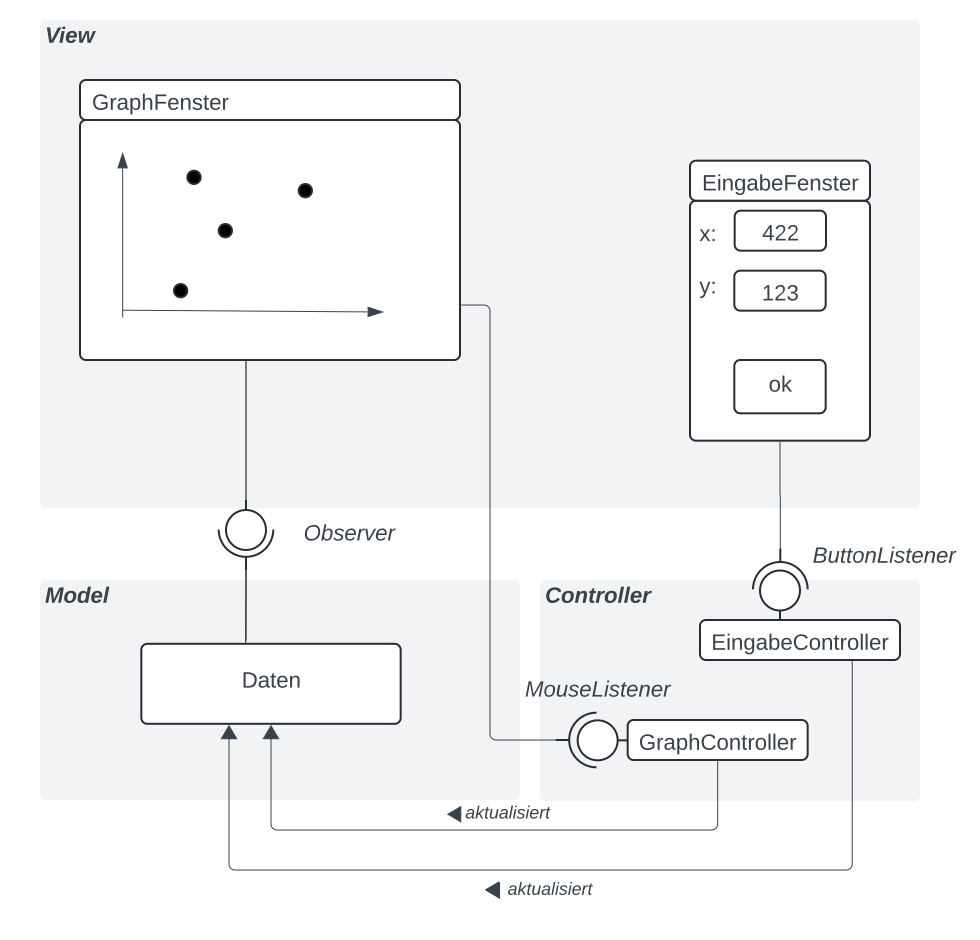
\includegraphics[scale=0.4]{chapters/aufgabe 8/img/mvc}
    \caption{Skizze des Zusammenspiels der in der Aufgabe 8 beschriebenen Komponenten.
    Die einzelnen Komponenten wurden ihrer Verantwortlichkeiten nach in die Bereiche \textit{Model}, \textit{View}, \textit{Controller} gruppiert. Für das \textit{GraphFenster} und das \textit{EingabeFenster} sind zwei verschiedene Controller angegeben, die unabhängig voneinander die Aktualisierung des Models vornehmen. (Quelle: eigene)}
    \label{fig:mvc}
\end{figure}